
\section{Molecular Imaging Methods}	% You can also have slides prior to the first section or work entirely without sections.

\begin{frame}[c]{Cryo-Electron Microscopy (Cryo-EM)}
    \begin{itemize}
        \item Major motivation
        \item Enables observation of molecules in near atomic resolution
        \item<2-> Observation through an electron microscope
        \item<2-> Frozen state of molecules required for observation
        \begin{itemize}
            \item<2-> Frozen molecules are fragile $\mapsto$ electron microscope low power
            \item<2-> During freezing, molecules rotate randomly
        \end{itemize}
        \item<2-> Observations can be reconstructed to a 3D model
        \item<2-> Single particle Cryo-EM 
    \end{itemize}
\end{frame}

\begin{frame}[c]{Cryo-Electron Microscopy (Cryo-EM) - Illustration}
    \only<1-2>{
        \begin{figure}
            \captionsetup[subfigure]{justification=centering}
            \centering
            \hfill
            \begin{subfigure}[t]{0.35\textwidth}
                \vskip 0pt
                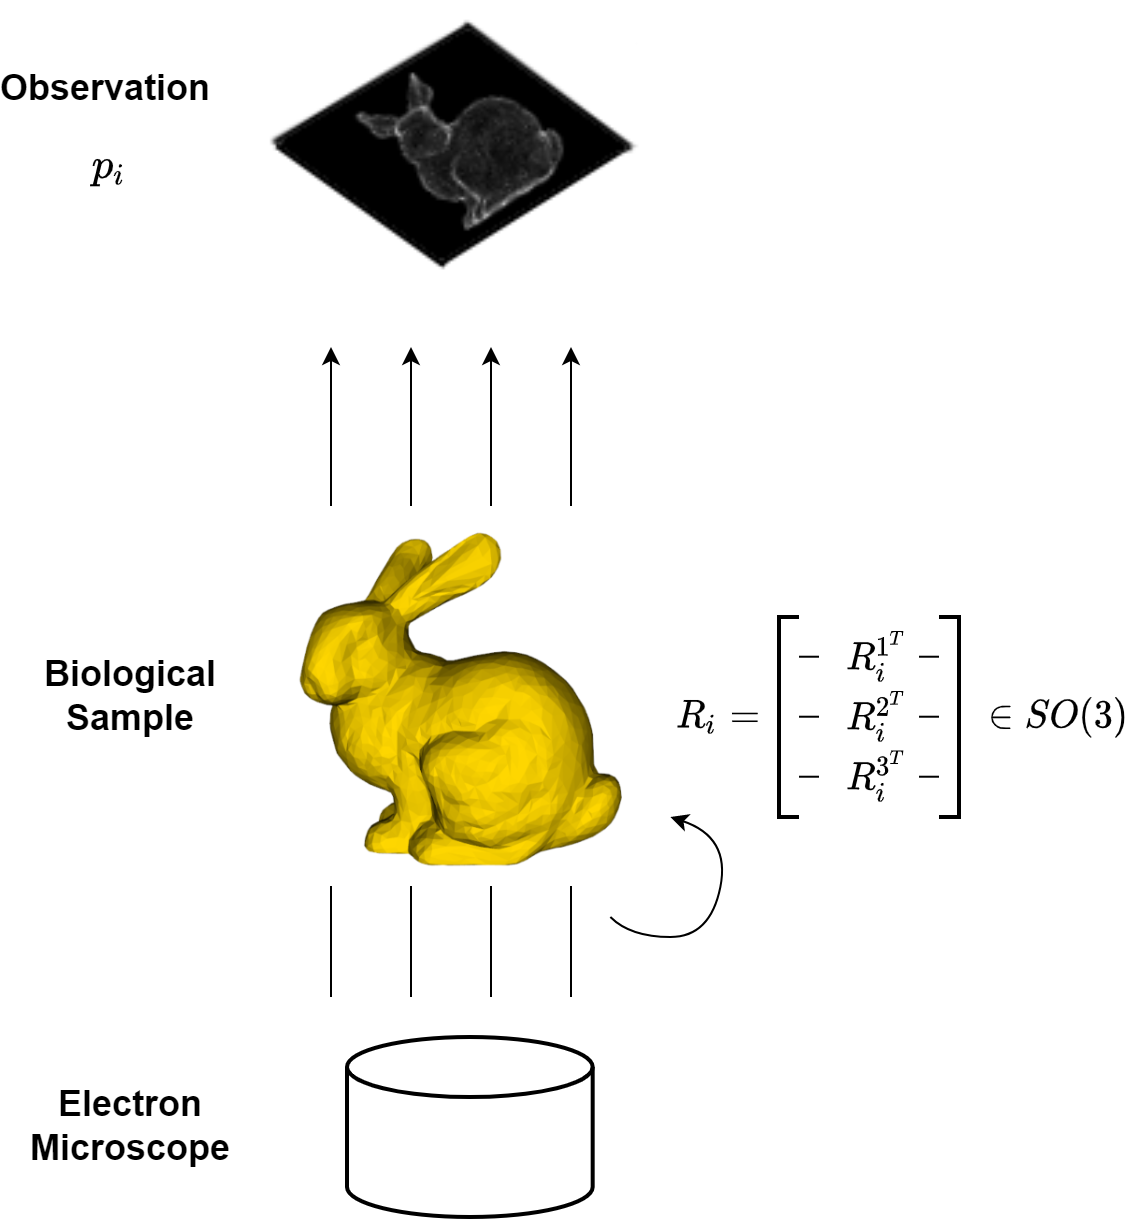
\includegraphics[width=\textwidth]{CryoObservation.drawio.png}
            \end{subfigure}\hfill
            \only<2>{
                \begin{subfigure}[t]{0.4\textwidth}
                    \vskip 0pt
                    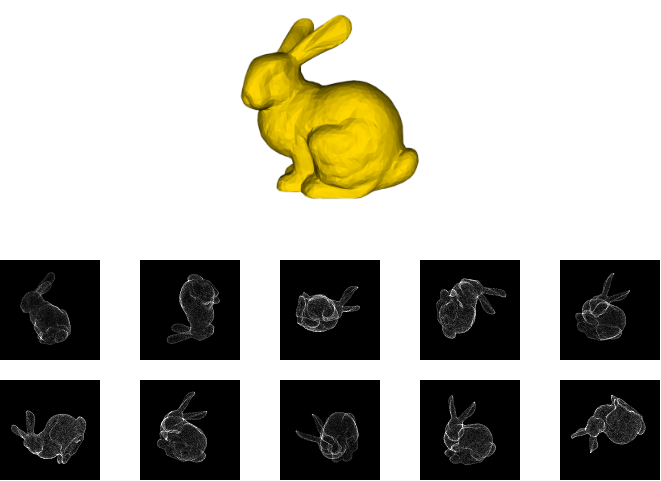
\includegraphics[width=\textwidth]{Cryo-EM_reconstruction.drawio.png}
                \end{subfigure}\hfill
            }
            \caption{Cryo-EM overview}
        \end{figure}
    
    }

    \only<3>{
        \begin{figure}
            \centering
            \begin{subfigure}[t]{0.4\textwidth}
                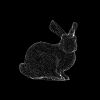
\includegraphics[width=\textwidth]{bunny_872.png}
                \caption{Clean micrograph}
            \end{subfigure}\hfill                
            \begin{subfigure}[t]{0.4\textwidth}
                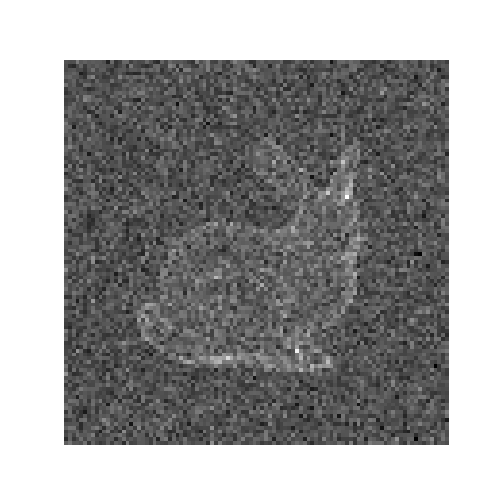
\includegraphics[width=\textwidth]{bunny_872_noisy.png}
                \caption{Noisy micrograph}
            \end{subfigure}\hfill                
        \end{figure}

    }
   
\end{frame}

%\begin{frame}
%    \begin{definition}[Cryo-EM observation]
%        $$ y_i[j,k] = \Pi_z (\; Rot(\;x; \theta_i))_{j,k} + \eta_i[j,k], \text{ with } 1 \leq i \leq N \text{ and } 1 \leq j,k \leq M,$$
%    \end{definition}
%    \begin{itemize}
%        \item $y_i[] \in \tilde{\Omega}, x \in L^2(\Omega)$ with $\Omega \subset \mathbb{R}^3 $ and $\tilde{\Omega} \subset \mathbb{R}^2 $
%        \item $M$ observation dimension
%        \item $\Pi_z : L^2(\Omega) \to L^2(\tilde{\Omega})$ projection operator
%        \item $Rot : L^2(\Omega) \to L^2(\Omega),$ is rotation operator
%        \item $Rot(x, \theta_i) = \left((x_1,x_2,x_3) \mapsto x( x_1R^1_{\theta_i}, x_2R^2_{\theta_i}, x_3R^3_{\theta_i})\right)$
%        \begin{itemize}
%            \item $\theta_i = [\theta_i^{(1)}, \theta_i^{(2)}, \theta_i^{(3)} ] $, with $\theta_i^{(1)}, \theta_i^{(2)}, \theta_i^{(3)} \in \mathbb{R}$
%            \item $R_{\theta_i} =  [R^1_{\theta_i}, R^2_{\theta_i}, R^3_{\theta_i}] \in SO(3)$ is the 3D rotation matrix 
%        \end{itemize}
%    \end{itemize}
%\end{frame}


\begin{frame}[c]{Computed Tomography (CT)}
    \pause
    \begin{columns}[c]
        \column{.55\textwidth}
            \begin{itemize}
                \item<2-> Similar to Cryo-EM
                \item<2-> Can be seen as a simpler version in 2D with known observation angles
                \item<2-> Good to start with towards a Cryo-EM algorithm
            \end{itemize}
        
        \column{.45\textwidth}
        \pause
        \begin{figure}
            \centering
            \begin{subfigure}[t]{0.45\textwidth}
                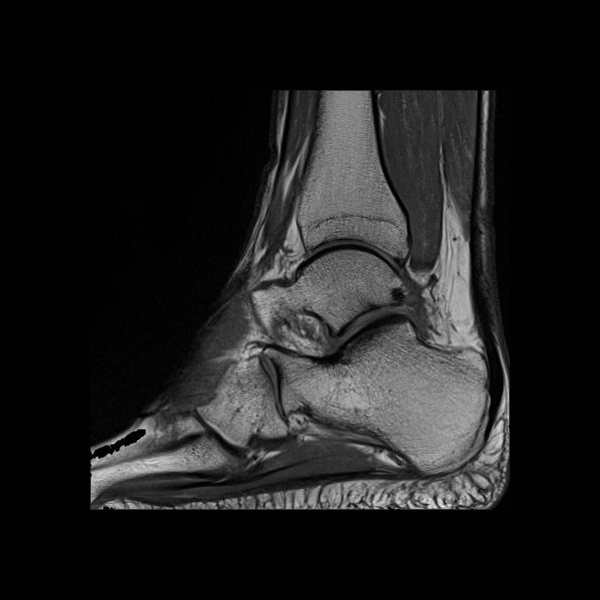
\includegraphics[width=\textwidth]{foot_cm}
                \caption{Biological sample}
            \end{subfigure}\hfill                
            \begin{subfigure}[t]{0.45\textwidth}
                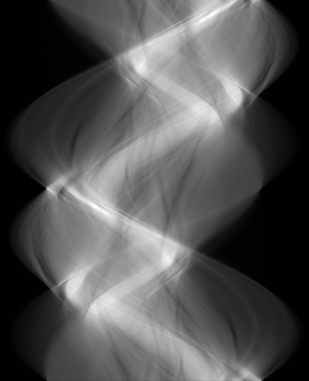
\includegraphics[width=\textwidth]{foot_sino}
                \caption{Clean observation (sinogram)}
            \end{subfigure}\hfill          
        \end{figure}

        
    \end{columns}
\end{frame}


\begin{frame}{Shared Observation Model}
    \pause

    \begin{block}{Observation}
        \only<2>{
            \begin{equation}
                \begin{aligned}
                    y_i &= p_i + \eta_i & \text{ with } 1 \leq i \leq N
                \end{aligned}
            \end{equation}
        }
        
        \only<3>{
            \begin{equation}
                \begin{aligned}
                    y_i &= p_i + \eta_i & \text{ with } 1 \leq i \leq N \\
                    y_i &=  A(x, \theta_i) +\eta_i  & \text{ with } 1 \leq i \leq N
                \end{aligned}
            \end{equation}
        }

    \end{block}
    \begin{columns}[T]
    \column{.42\textwidth}

    
    \begin{itemize}
        \item<2-> \alert<2>{$y$: noisy observation}
        \item<2-> \alert<2>{$p$: noiseless observation}
        \item<2-> \alert<2>{$\eta$: noise, assumed  $\eta_i \sim \mathcal{N}(0,\sigma^2)$}
        \item<3-> \alert<3>{$x$: biological sample}
    \end{itemize}
        
    \column{.58\textwidth}

    \begin{itemize}
        \item<2-> \alert<2>{$y_i \in \mathbb{R}^M, $ $M$: observation dimension}
        \item<2-> \alert<2>{$N$: number of observations}
        \item<3-> \alert<3>{$A: x \mapsto A(x; \theta_i) \in \mathbb{R}^M$: a non-linear operator}
        \item<3-> \alert<3>{$\theta_i$: observation angle}
    \end{itemize}

    \end{columns}
    
\end{frame}

\begin{frame}{Observation - Illustration }

    \begin{figure}
    \centering
    \begin{subfigure}{0.25\textwidth}
        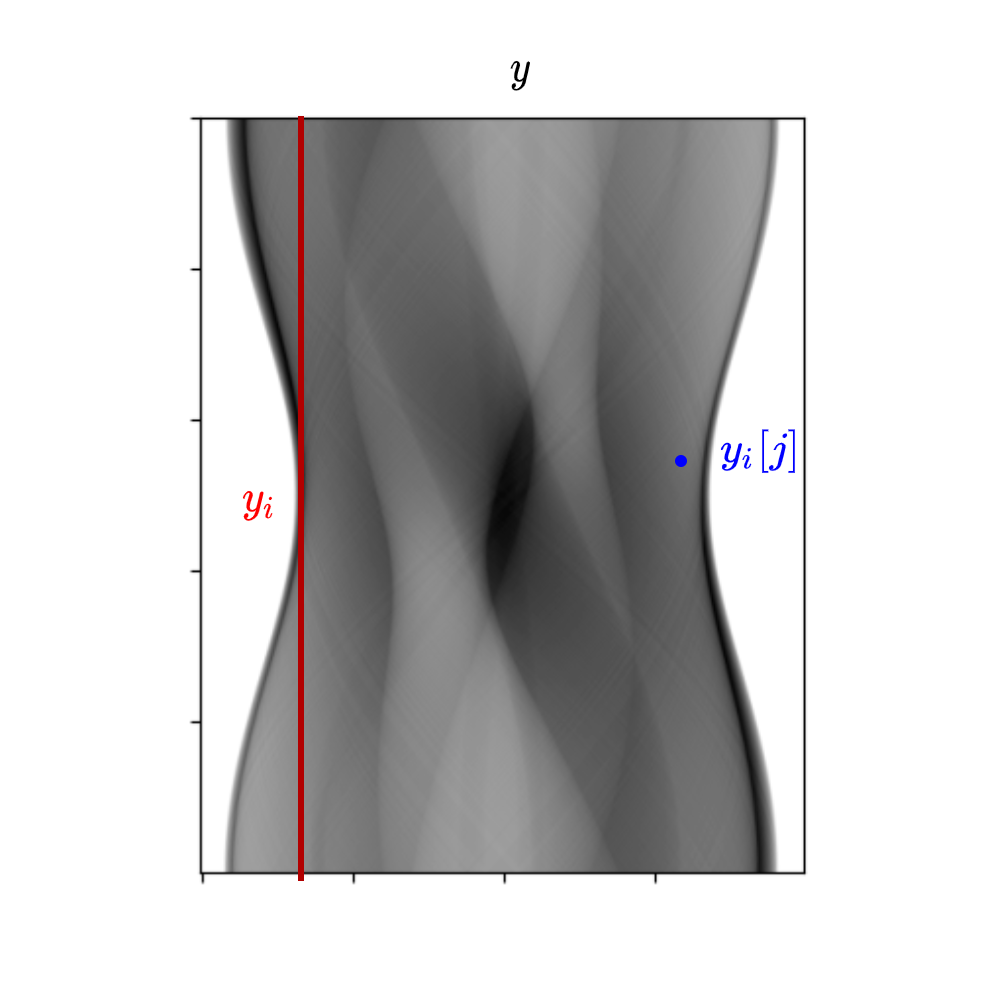
\includegraphics[width=\textwidth]{sino_yi.drawio.png}
        \caption{CT Observation - sinogram}
    \end{subfigure}
    \begin{subfigure}{0.6\textwidth}
        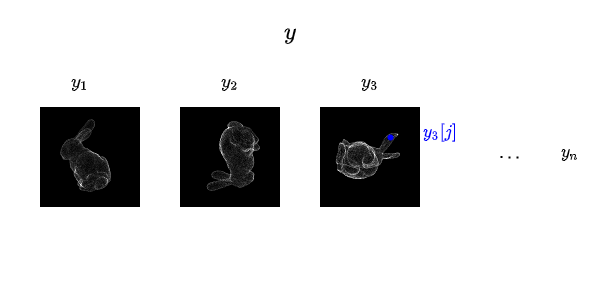
\includegraphics[width=\textwidth]{micrograph_yi.drawio.png}
        \caption{Cryo-EM Observation - micrographs}
    \end{subfigure}
\end{figure}

\end{frame}


\begin{frame}{Reconstruction}
    \pause
  
    \begin{block}{Reconstruction}
        \begin{equation}
            \begin{aligned}
                \textit{Recon} : & \mathbb{R}^{M \times N} \to \mathbb{R}^{M \times M} & y \mapsto Recon(y; \theta)
            \end{aligned}
        \end{equation}
    \end{block}
\end{frame}



\begin{frame}{Signal-to-noise-ration (SNR)}
    \pause
    \begin{itemize}
        \item SNR is a measure, which compares the power of an input signal to the power of the undesired noise
        \item Typically given in decibel (dB)
        \item SNR $\le 0$ dB indicates more noise than signal 
    \end{itemize}


    \begin{tcolorbox}[colback=red!5!white,hide=<1-2>, alert=<3>, colframe=red!75!black]
        $SNR_y$ is used to define the level of noise in an observation.
    \end{tcolorbox}

        
    \begin{tcolorbox}[colback=red!5!white,hide=<1-3>, alert=<4>, colframe=red!75!black]
        $SNR$ is used as a metric for the quality of reconstructions.
    \end{tcolorbox}

\end{frame}



\begin{frame}{Reconstruction -  Computed Tomography}
    \begin{columns}
        \column{.45\textwidth}
        
        \begin{itemize}
            \item Filter Backprojection (FBP)
            \begin{itemize}
                \item Can be considered historical approach
                \item Enables reconstruction for moderate noise
            \end{itemize}
            \item<3> Neural Network Approaches
            \begin{itemize}
                \item Today state-of-the art
                \item Using result of FBP and further denoise
                \begin{itemize}
                    \item U-Net \cite{unet-tomography}
                \end{itemize}
            \end{itemize}
        \end{itemize}

        \column{.55\textwidth}

        \only<2->{
            \begin{figure}
                \centering
                \begin{subfigure}[t]{0.45\textwidth}
                    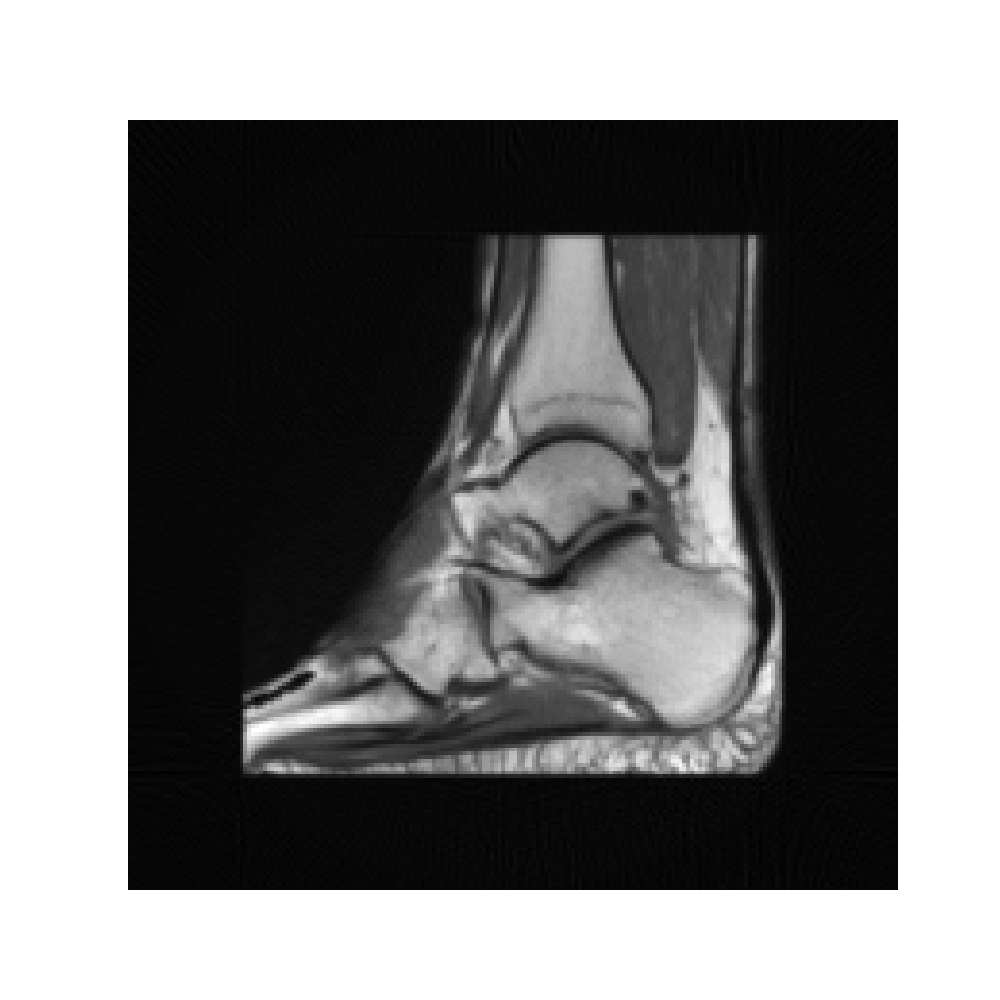
\includegraphics[width=\textwidth]{foot_reco_clean.png}
                    \caption{Reconstruction clean: \\
                        $Recon(p, \theta) \approx x$}
                \end{subfigure}
                \begin{subfigure}[t]{0.45\textwidth}
                    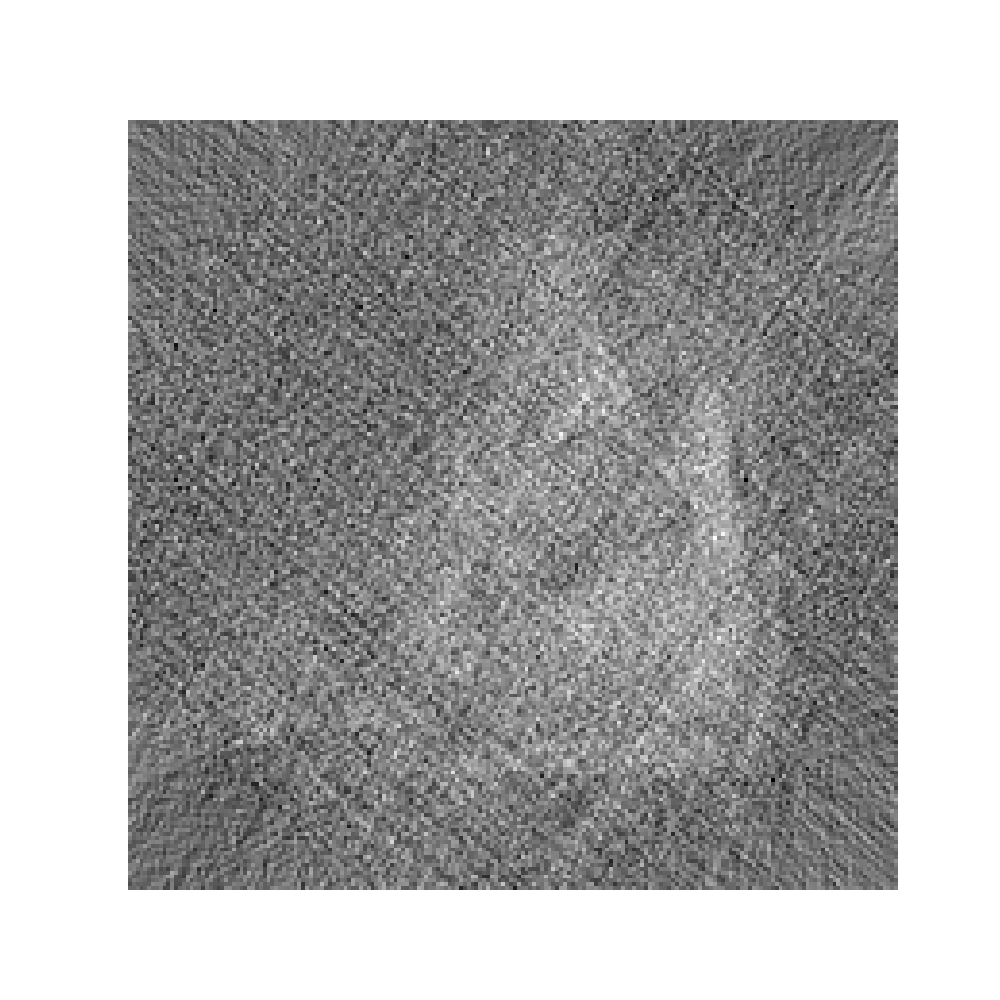
\includegraphics[width=\textwidth]{foot_reco_snr_5.png}
                    \caption{Reconstruction noisy with $SNR_y$ 5 dB: \\
                        $Recon(y, \theta) \not\approx x$}
                \end{subfigure}
            \end{figure}
        }
    \end{columns}
\end{frame}



\begin{frame}{Problem and Goal}
    \pause
    \begin{block}{Problem}
        $p$ not observable directly only access to $y$.
    \end{block}
    \pause
    \begin{block}{Goal}
        $$ denoiser:   y_i \mapsto y_i^* \approx p_i $$
        $$ \textit{Recon} \left( denoiser(y; \theta) \right) \approx x $$
    \end{block}

\end{frame}


